\documentclass[conference]{IEEEtran}
\IEEEoverridecommandlockouts
% The preceding line is only needed to identify funding in the first footnote. If that is unneeded, please comment it out.
\usepackage{amsmath,amsthm,amssymb} %modos matemáticos y  simbolos
\usepackage{latexsym,amsfonts} %simbolos matematicos
\usepackage{cancel} %hacer la linea que cancela las ecuaciones
\usepackage[spanish, es-noshorthands]{babel} %comandos en español y cambia el cuadro por la tabla
\decimalpoint %cambia las comas por puntos decimal
\usepackage[utf8]{inputenc} %caracteristicas del español
\usepackage{physics} %Simbolos fisicos
\usepackage{array} %mejores formatos de tabla
\parindent =0cm %sangria 
\usepackage{algorithmic}
\usepackage{graphicx}
\usepackage{textcomp}
\usepackage{xcolor}
\usepackage{mathtools} 
\usepackage[framemethod=TikZ]{mdframed}%Entornos talegas
\usepackage[colorlinks = true,
			linkcolor = blue,
			citecolor = black,
			urlcolor = blue]{hyperref}%formato de los links y URL's
\usepackage{multicol} %varias columnas
\usepackage{enumerate} %enumeraciones
\usepackage{pgf,tikz,pgfplots} %documentos en formato tikz
\usepackage{mathrsfs} %letras chingonas (transformada de laplace)
\usepackage{subfigure} %varias figuras seguidas
\usepackage{tabulary}
\usepackage{multirow} %ocupar varias filas en una tabla
\usepackage{fancybox} %recuadros talegas
\usepackage{float} %ubicar graficas
\usepackage{color}
\usepackage{comment}
\usepackage{stackrel}
\usepackage{calligra}
\usepackage{lipsum}
\usepackage{cite}
%\pgfplotsset{compat=1.17} 

\newcommand{\R}{\mathbb{R}}
\newcommand{\Z}{\mathbb{Z}}
%%%%%%%%%%%%%%%%%%%%%%%%%%%%%%%%%%%%%%%%%%%%%%%%%%%%%%
\def\BibTeX{{\rm B\kern-.05em{\sc i\kern-.025em b}\kern-.08em
    T\kern-.1667em\lower.7ex\hbox{E}\kern-.125emX}}
\begin{document}



%%% CARÁTULA
\begin{titlepage}



\begin{flushleft}
    Universidad de San Carlos de Guatemala \\
    Escuela de Ciencias Físicas y Matemáticas \\
    Curso: Laboratorio de Instrumentación \\
    Profesor: Wendy Miranda
\end{flushleft}

\vspace{6cm}

\begin{center}
    \huge{Motor \textit{Brushless}} y Sensor CNY$70$ \\[1cm]
    \large{Tarea 3 y Complementaria}
\end{center}

\vspace{10.5cm}

\begin{flushright}
    Diego Sarceño \\
    $201900109$
\end{flushright}

\vspace{0.5cm}

\begin{center}
    Guatemala, 03 de noviembre del 2022
\end{center}

\end{titlepage}



\section{Introducción}
    En esta práctica se modela un motor brushless con un sensor de efecto hall. Y el uso de fototransistores en forma del sensor CNY70, para ver los cambios mediante un LED y un motor, lo que demuestra su equivalencia a switches/interruptores.


\begin{IEEEkeywords}
    CNY70, 2N2222, Efecto hall, transistores.
\end{IEEEkeywords}

\section{Objetivos}

\subsection{General}
    \begin{enumerate}[1.]
        \item Poder analizar y comprender las aplicaciones del sensor de efecto hall y del sensor CNY70.
    \end{enumerate}
\subsection{Específicos}
    \begin{enumerate}
        \item Poder simular y analizar circuitos con transistores y los respectivos sensores.
    \end{enumerate}
%\section{Introducción}
    
\section{Marco Teórico}
\subsection{Efecto Hall}
Es un fenomeno que se caracteriza por la aparición de un campo electrico por la separación de cargas en el interior de un conductor con corriente cirunlando y un campo magnético. \\\\
El sensor \textbf{US1881KUA} está compuesto por un regulador de voltaje, un sensor de efecto hall con cancelación dinámica, un generador Schmitt y un controlador de salida de drenaje abierto. Este dispositivo consta de 3 patas (VDD, GND y el output) y funciona como una especie de switch bajo la presencia de un campo magnetico (específicamente un polo).

\subsection{Fototransistor CNY70}
Este dispositivo esta conformado por un emisor de infrarrojos y un fototransistor, todo esto, recubierto de un material que bloquea perfectamente la luz visible. Los fototransistores son típicamente NPN, los cuales no tienen patilla conectada a la base, la cual está agrandada y sensible a la luz.



    
%\section{Diseño Experimental}
%    \subsection{Materiales a Utilizar}
%        \begin{itemize}
%    	\item 
%    \end{itemize}
%
%    \subsection{Procedimientos}
%        \begin{enumerate}
%            \item 
%        \end{enumerate}
\section{Resultados}
\subsection{Motor Brushless}
De la implementación del motor brushless, se hizo girar un iman a $60rpm$, con esto se midieron los cambios de voltaje con un osciloscopio y, como era de esperarse, se tiene un voltaje oscilante por cada vez que el campo magnético se incrementa en cada revolución.

\begin{figure}[H]
	\centering
	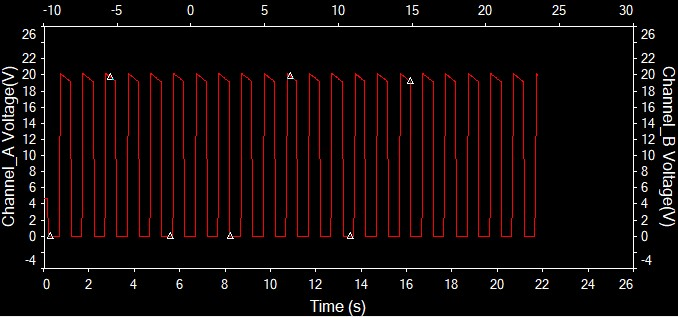
\includegraphics[scale=0.5]{./img/brushless_graph.jpeg}
	\caption{Voltaje oscilante del motor brushless.}
	\label{brushcirc}
\end{figure}
    
\section{Discusión de Resultados}
\begin{enumerate}
    \item Al momento de que se detecte luz infrarroja se envía corriente a la base, haciendo una función de botón enviando todo a tierra y apagando el led y viceversa.
   	\item En el ejercicio 2, el transistor funciona con un switch, que limita/permite el paso de corriente lo que hace funcionar el motor.
\end{enumerate}
\section{Conclusiones}
\begin{enumerate}
    \item El sensor hall se activa mendiante la aplicación de un campo magnético, con lo que podemos volver una corriente directa en una oscilate, dependiente de la frencuencia de cambio del cambio magnético.
    \item El sensor CNY70 funciona como un switch no mecánico, el cuál es accionado por una señal infrarroja.
\end{enumerate}
%\section{Recomendaciones}

\section{Anexos}
\subsection{Circuitos}
\begin{figure}[H]
	\centering
	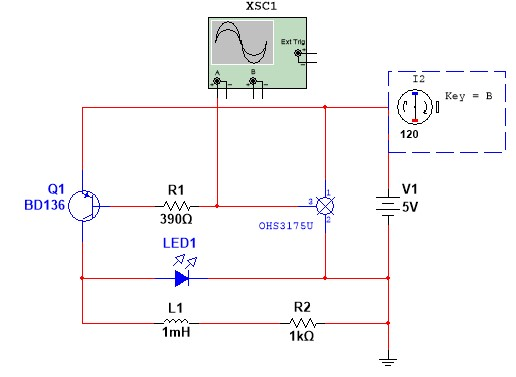
\includegraphics[scale=0.6]{./img/brushless.jpeg}
	\caption{Implementación del motor Brushless bajo el equivalente del sensor US1881KUA.}
	\label{brushcirc}
\end{figure}



\begin{figure}[H]
	\centering
	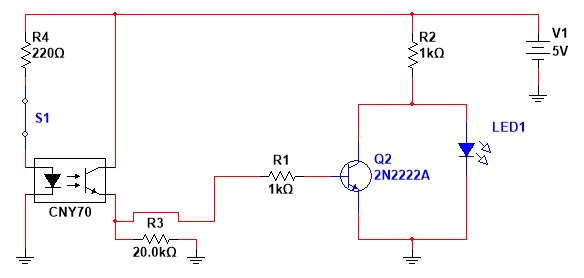
\includegraphics[scale=0.6]{./img/ej1.jpeg}
	\caption{Interruptor simple utilizando el sensor CNY70 y el transistor 2N2222.}
	\label{ej1}
\end{figure}



\begin{figure}[H]
	\centering
	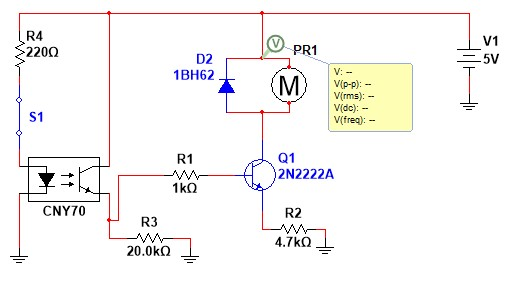
\includegraphics[scale=0.6]{./img/ej2.jpeg}
	\caption{Motor activado por los sensores CNY70 y el transistor 2N2222.}
	\label{ej2}
\end{figure}

\subsection{Cálculos}
\subsubsection{Brushless}
Para esta implementación, se tiene la siguiente ecuación
	$$ i = \frac{\text{VCC} - \text{VCE}}{R}. $$



\begin{thebibliography}{00}
\bibitem{b1} Neamen, D. A. (2007). \textit{Microelectronics: circuit analysis and design} (Vol. 43). New York: McGraw-Hill.
\bibitem{b2} 2021. \textit{Circuit Diagram}. \url{https://www.circuit-diagram.org/}
\end{thebibliography}

\end{document}